\chapter{Információs technológiai infrastruktúrák}
\section{A klasszikus IT infrastruktúra}
A klasszikusnak mondott IT infrastruktúrát az írás korábbi részében már bemutattam. Itt most a háromrétegű architektúra egyes rétegeinek skálázását, megbízhatósági szintjének növelésére adott lehetőségeket szeretném bemutatni.
\subsection{Adatbázis réteg}
\todo{Klaszterek, replikák, stb.}
\subsection{Alkalmazás réteg}
\todo{PHP, Java skálázás?}
\subsection{Webkiszolgáló réteg}
\todo{Loadbalancing} 
\section{Felhőalapú infrastruktúrák}
\subsection{Mi is az a ,,számítási felhő''?}

A ,,számítási felhő'' (angolul \foreignlanguage{english}{cloud computing}) egy modell kényelmes, hálózaton keresztül hozzáférhető, konfigurálható számítási erőforrások (pl. hálózat, szerverek, tárhelyek, alkalmazások és szolgáltatások) egy megosztott készletének elérhetőségére, mely erőforrásokat minimális intézkedési erőfeszítéssel vagy szolgáltatói közbenjárással gyorsan rendelkezésre lehet bocsátani \cite{nistsp800-145}.

\todo{Lehet, hogy még finomítani kell a fordításon!}

\begin{comment}
Cloud computing is a model for enabling ubiquitous, convenient, on-demand network access to a shared pool of configurable computing resources (e.g., networks, servers, storage, applications, and services) that can be rapidly provisioned and released with minimal management effort or service provider interaction. 
\end{comment}

Általában hivatkozás szintjén nincsenek elkülönítve az Interneten keresztül szolgáltatott alkalmazások, és a felhő infrastrukturális részét képező hardverek, szoftverek, amelyek ezeket az alkalmazásokat elérhetővé teszik. Ahogy azt \aref{fig:cloud_computing_hu}.~ábrán is szemléltetni próbálom a felhő részét képezi az alkalmazás, szolgáltatás, és a hardver is.

\begin{figure}[h!]
\centering
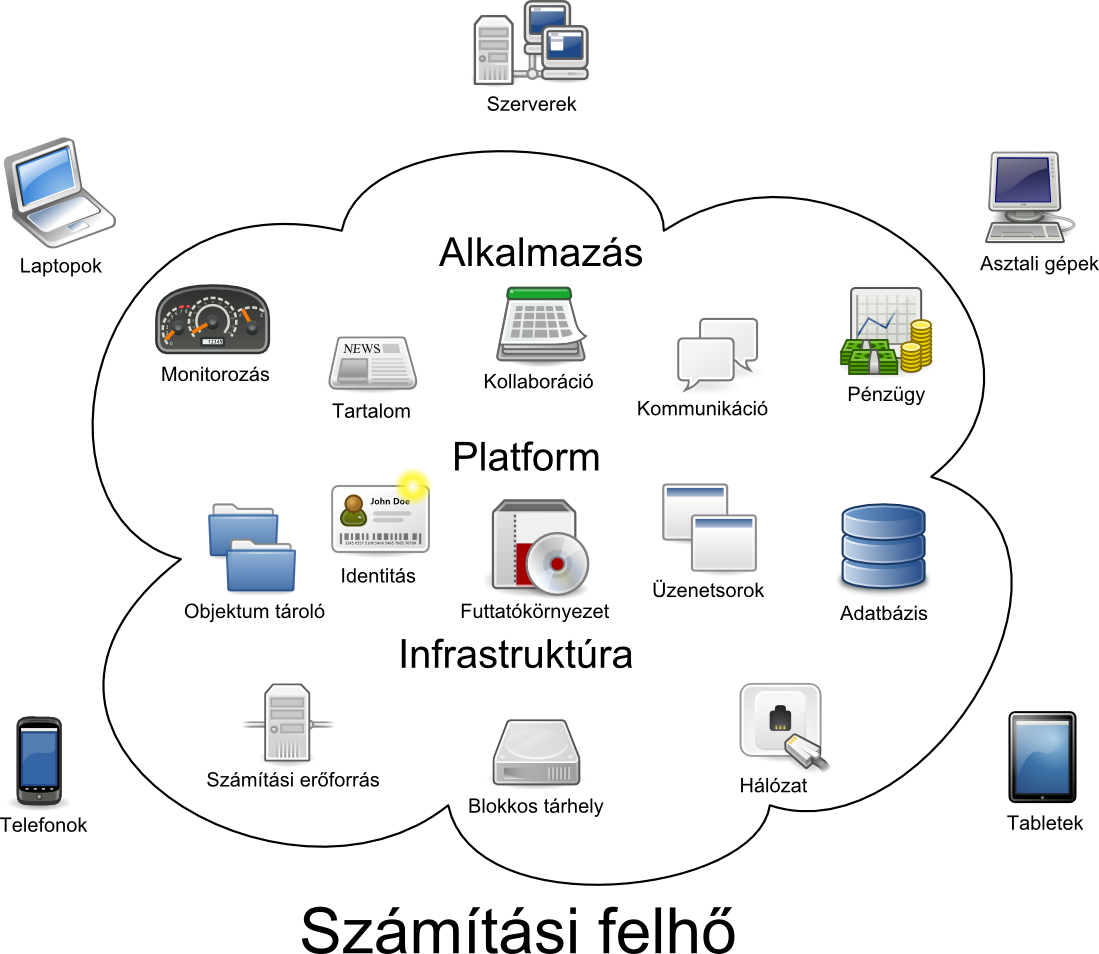
\includegraphics[width=1.0\textwidth]{figures/Cloud_computing_hu.png}
\caption{A számítási felhő (\foreignlanguage{english}{cloud computing}) (Forrás: \href{https://en.wikipedia.org/wiki/File:Cloud\_computing.svg}{Wikipedia})} \label{fig:cloud_computing_hu}
\end{figure}

\todo{Object Storage ?= Objektum tároló}

\todo{Queue ?= Üzenetsorok}

\todo{Runtime ?= Számításelosztás}

Mélyebb elemzés során azonban a felhőt rétegekre lehet bontani, amely rétegeket a következő alfejezetben részletezném.

\subsection{A felhő rétegei}
A felhő napjainkban négy architekturális rétegből épül fel, amelyeket alulról fölfelé érdemes megvizsgálni.
 
\subsubsection{Adattár, mint szolgáltatás (\foreignlanguage{english}{data-Storage-as-a-Service, dSaaS})}
\subsubsection{Infrastuktúra, mint szolgálatás (\foreignlanguage{english}{Infrastructure-as-a-Service, IaaS})}
\subsubsection{Platform, mint szolgáltatás (\foreignlanguage{english}{Platform-as-a-Service, PaaS})}
\subsubsection{Szoftver, mint szolgáltatás (\foreignlanguage{english}{Software-as-a-Service,SaaS})}
